\newpage
\section{Analysis and Design 2}
The design \nameone is fully functional; the aim of the second design \nametwo is to improve upon it. There are a few issues with the first design. To begin with, it is not portable. That makes it impossible to wear and move freely in the virtual environment. Secondly, the movement of the finger pads of the exoskeleton is circular; it does not capture the trajectory or normal forces of the simulated robot gripper well. A more sophisticated solution would be a gripper-like exoskeleton \cite{dai2023gripper} as discussed in the background, but incorporating force feedback. Lastly, the exoskeleton could be lighter. The two-motor design is heavy and would be uncomfortable to wear. The proposed alternative is to use only one motor instead of two, as pinching can be designed as a linear motion with one DOF. Such a design would save on costs and weight. Also, a smaller motor could be utilized. With these goals in mind, the ideation phase began; many ideas were brainstormed (for some of the examples, see appendix \ref{appendix:gripper-ideation-phase}). The final design is inspired by how some of the robotic grippers work, using only one motor and implementing the principle of double rack and pinion (Fig. \ref{fig:second_exoskeleton}, Appendix \ref{appendix:exoskeleton-engineering-drawings}). The global position tracking is achieved with the use of a standard VR controller in order to minimize costs. The controller holder was designed in Blender by using a boolean operator to subtract the shape of the hand and the controller from a cuboid mesh. Then it was 3D printed and hot-glued to a half-finger glove. The controller is secured using Velcro straps. The local position tracking is obtained from the positional data of the motor. The casing around the motor and rack and pinion were designed using Autodesk Inventor and 3D printed as well. The hole for the thumb is rotated at 45$^{\circ}$ for increased comfort. One side is extruded to rest against the palm of the hand, and the exoskeleton is secured using another Velcro strap. Some of the standard parts were bought instead of being manufactured. Screws, brass inserts, and a linear guide with rails that is used to reduce the friction and stabilize the linear movement. All of this put together results in a simple, lightweight, and affordable exoskeleton design. The \nametwo parts and prices can be seen in Table \ref{table:exoskeleton-2-parts}.

\begin{table}[ht]
  \setlength{\abovecaptionskip}{6pt}
  \centering
  \begin{tabular}{|l|c|c|}
  \hline
  \multicolumn{1}{|c|}{\textbf{Description}} & \textbf{Quantity}                  & \textbf{Toal Price} \\ \hline
  \multicolumn{3}{|l|}{\textbf{Screws}} \\ \hline
  M2 x 8mm              & 8               & 7.5 DKK        \\ \hline
  M2.5 x 14mm              & 4               & 15 DKK        \\ \hline
  M2.5 x 8mm              & 4               & 7.5 DKK        \\ \hline
  M3 x 8mm              & 16               & 15 DKK       \\ \hline
  \multicolumn{3}{|l|}{\textbf{Brass Inserts}} \\ \hline
  M3 x 5mm, OD 4.5mm              & 16               & 20 DKK        \\ \hline
  \multicolumn{3}{|l|}{\textbf{Mechanical Parts}} \\ \hline
  100mm linear guide & 1 & 24 DKK  \\ \hline
  MGN7C slider & 2 & 120 DKK  \\ \hline
  Half finger gloves & 1 & 20 DKK \\ \hline
  Hook and loop fastener & 2 & 22 DKK \\ \hline
  \multicolumn{3}{|l|}{\textbf{Electronics}} \\ \hline
  Dynamixel XM430-W350-R & 1 & 2140 DKK \\ \hline
  SMPS2Dynamixel Power Adapter & 1 & 50 DKK \\ \hline
  U2D2 & 1 & 280 DKK \\ \hline
  \multicolumn{3}{|l|}{\textbf{3D Print}} \\ \hline
  Polylactic Acid (PLA) filament & 300g & 60 DKK \\ \hline
  & & \textbf{2781 DKK (372.76 €)} \\ \hline
  \end{tabular}
  \caption{\nametwo Exoskeleton Parts}
  \label{table:exoskeleton-2-parts}
\end{table}

\begin{figure}[ht]
  \centering
  \begin{subfigure}{0.45\textwidth}
      \centering
      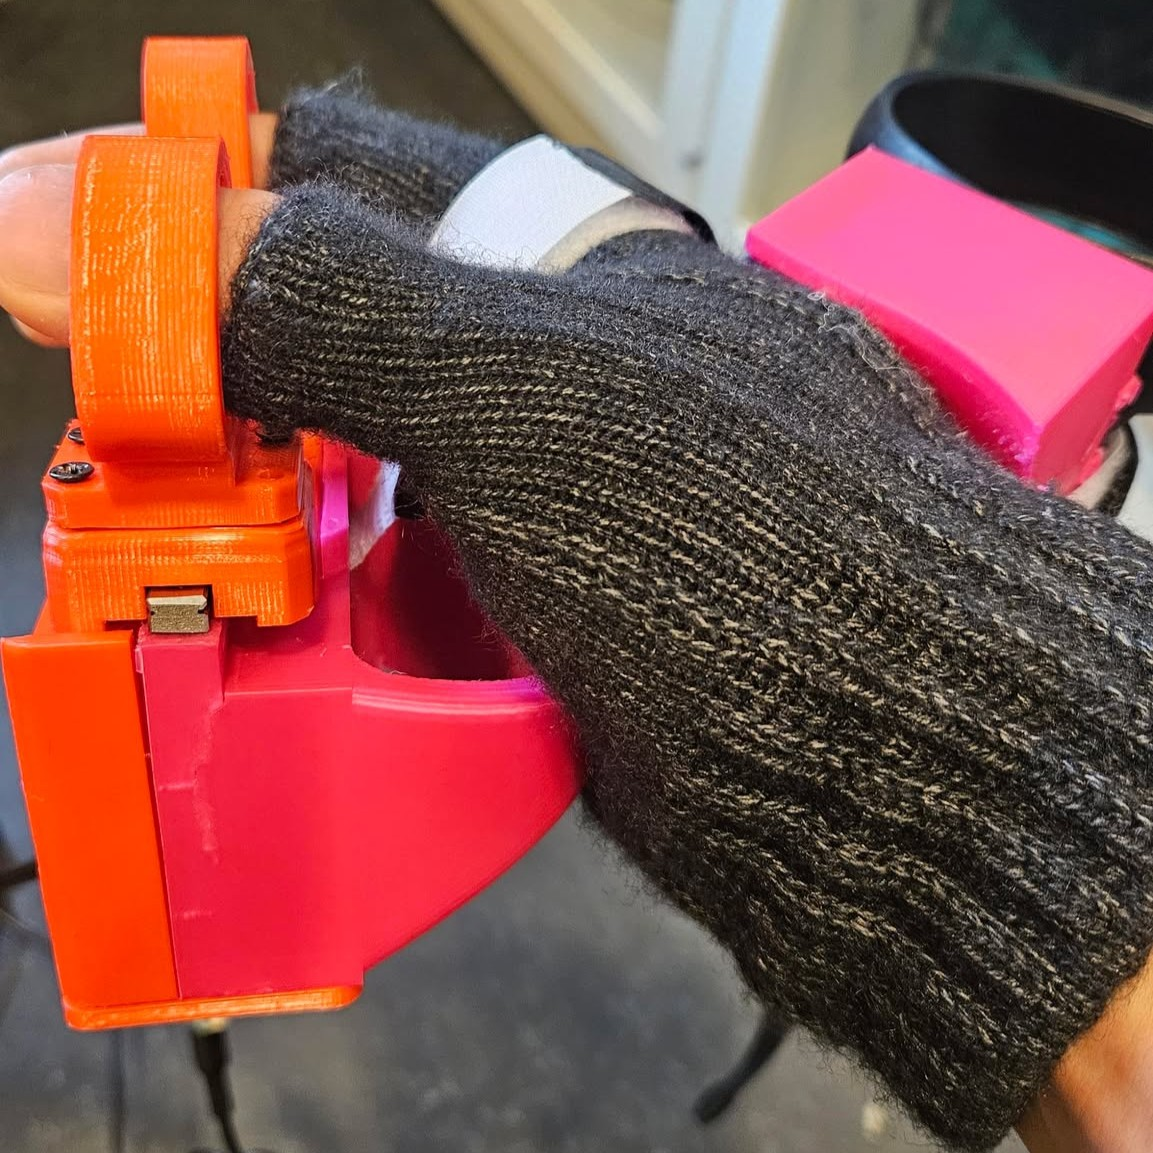
\includegraphics[width=\linewidth]{chapters/exoskeleton/images/design/side.jpg}
  \end{subfigure}
  \begin{subfigure}{0.45\textwidth}
      \centering
      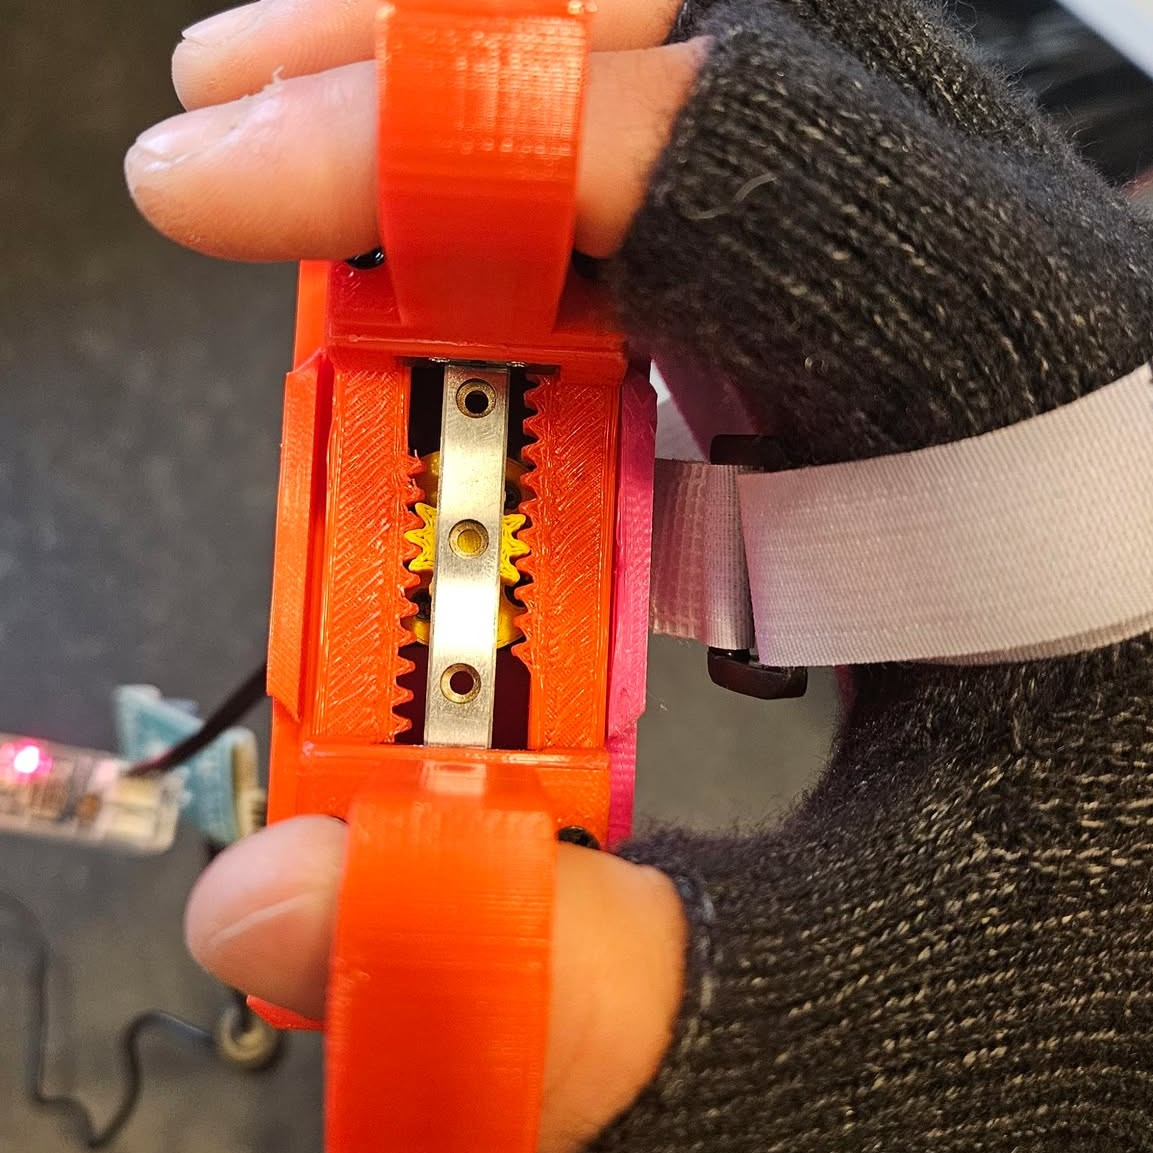
\includegraphics[width=\linewidth]{chapters/exoskeleton/images/design/top.jpg}
  \end{subfigure}
  \begin{subfigure}{0.45\textwidth}
      \centering
      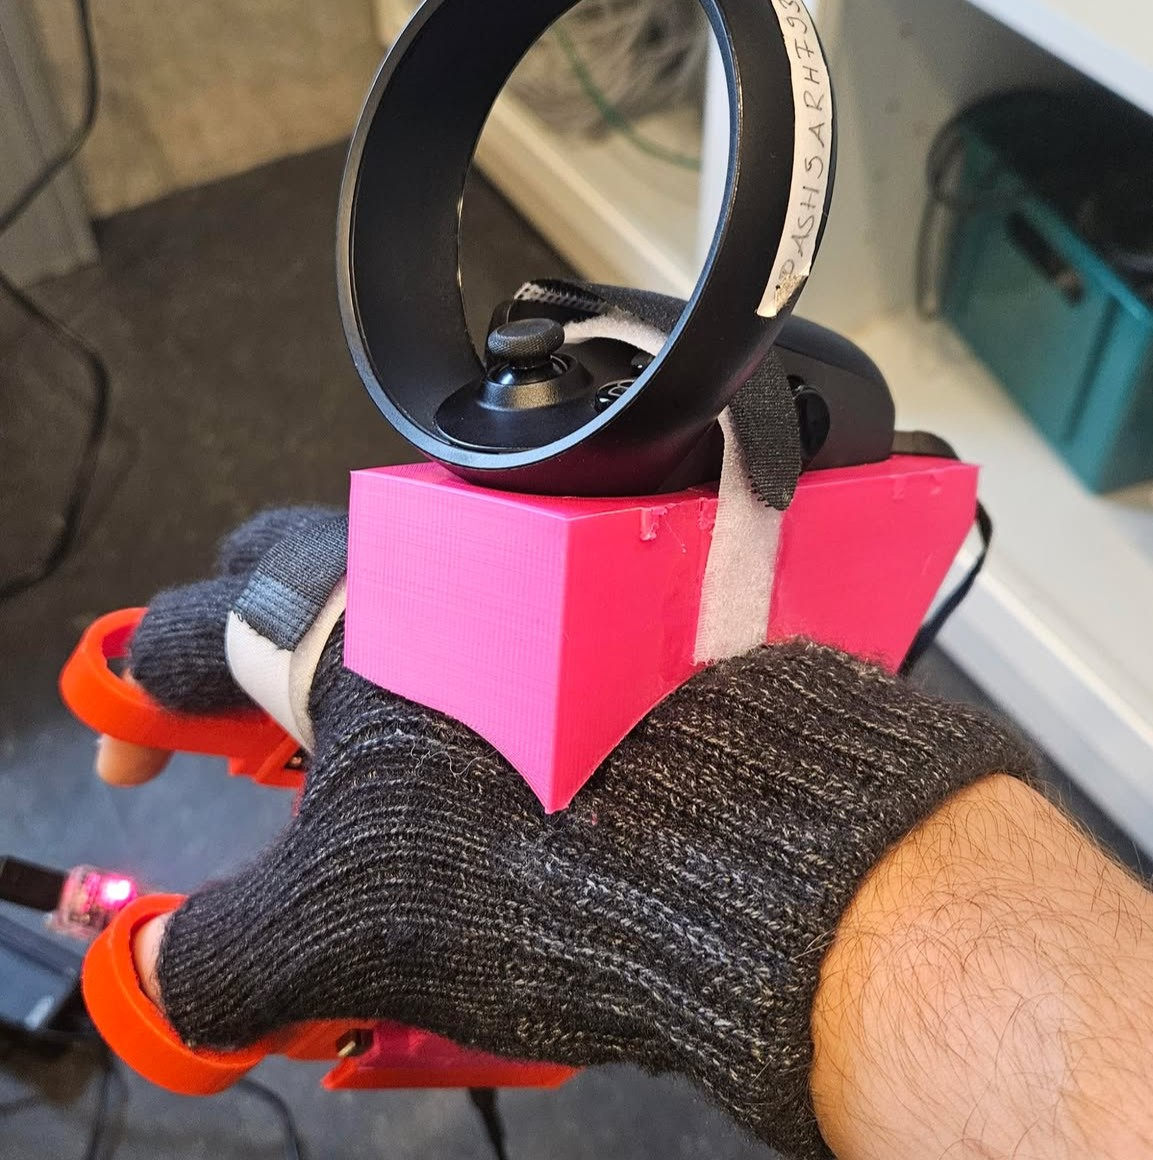
\includegraphics[width=\linewidth]{chapters/exoskeleton/images/design/controller_side.jpg}
  \end{subfigure}
  \begin{subfigure}{0.45\textwidth}
      \centering
      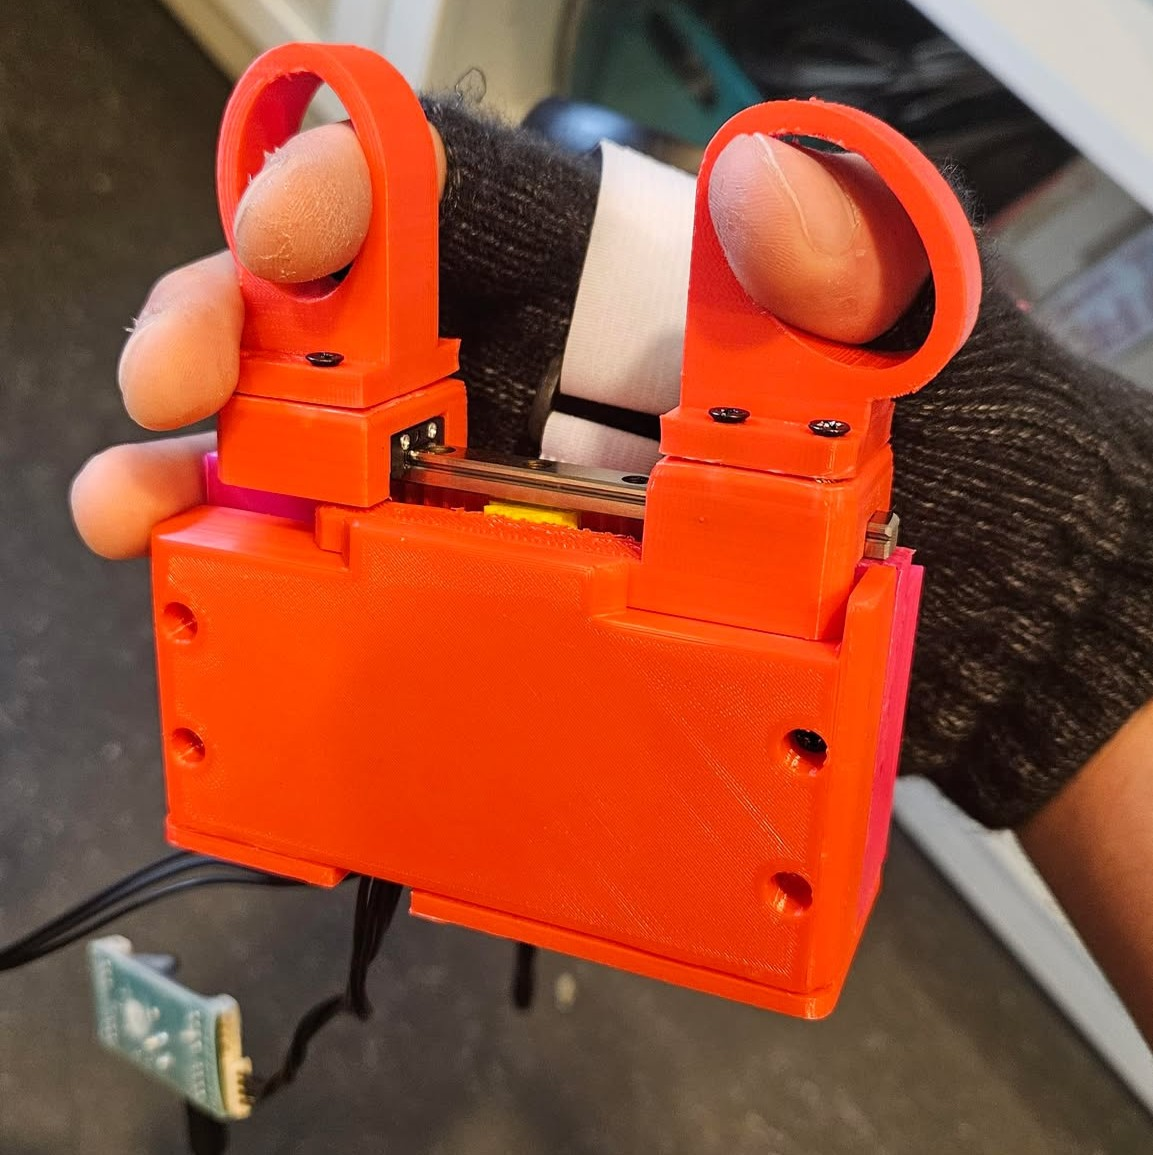
\includegraphics[width=\linewidth]{chapters/exoskeleton/images/design/back.jpg}
  \end{subfigure}
  \caption{\nametwo Exoskeleton}
  \label{fig:second_exoskeleton}
\end{figure}
